\section{The Limits of Measurement: When Sets Bite Back (1960)}

\section{From Atomism to Axioms: Russell, Hilbert, and the Dream of Formalization}

By the early 20th century, a group of mathematicians known as the \textbf{Formalists}---led by \textbf{David Hilbert}---dreamed of turning mathematics into a kind of perfect machine. The goal? To formalize all of math into a neat list of axioms and rules, so that every mathematical truth could be derived mechanically, like running a program. No ambiguity. No mystery. Just logic, grinding forward with total reliability.

Hilbert famously declared: \textit{``We must know. We will know.''} Mathematics, in his vision, would become a closed system: all truths could be proven, and all proofs could be checked by following the rules.

This belief wasn’t limited to mathematicians. It resonated with a broader intellectual movement known as \textbf{logical positivism}, led by philosophers like \textbf{Rudolf Carnap} and the \textbf{Vienna Circle}. Logical positivists believed that all meaningful statements could either be verified empirically (through observation) or proven logically (through deduction). Mathematics, to them, was the purest expression of this ideal: a universe of perfect clarity, built from self-evident axioms and strict logical steps. If we could formalize math, they argued, we could anchor all of science and reasoning on unshakable foundations.

But there was a deeper question lurking behind all of this: \textit{How do we know what’s true—or even what’s right or wrong?} People often assume we always know. Not so. And in the early 20th century, this uncertainty reached even into mathematics.

Enter \textbf{Bertrand Russell}.

Russell proposed an ambitious idea called \textbf{logical atomism}. The goal was to break down all mathematical concepts and arguments into tiny, irreducible logical units---``atoms'' of reason---and then show that they could all be derived from pure logic. It was a philosophical chain reaction waiting to happen.

Unfortunately, it didn’t quite work out that way.

After years of painstaking effort, Russell---alongside Alfred North Whitehead---produced the monumental \textit{Principia Mathematica}. But instead of reducing mathematics to pure logic, it revealed how staggeringly difficult that task really was. Still, it was a landmark. \textit{Principia} didn’t solve the problem, but it deeply influence \textbf{Hilbert}, and changed the course of mathematical logic.

It was, in a way, the mathematical equivalent of what physicists did when they split the atom: an attempt to reduce the complex to its fundamental components. In physics, splitting the atom led to a new kind of energy and a new kind of danger. In mathematics, analyzing these logical ``atoms'' led to a new kind of mathematics altogether.

Hilbert approached the problem from a completely different angle. Instead of trying to reduce mathematics to logic, he asked: \textit{What must a foundational system for mathematics be like if we want it to work at all?}

His answer came in the form of three key requirements:

\begin{enumerate}
    \item \textbf{Consistency} – The system must not produce contradictions.
    \item \textbf{Completeness} – Every true mathematical statement must be provable within the system.
    \item \textbf{Decidability} – There must be a definite procedure, a mechanical method, to determine whether any given statement is provable.
\end{enumerate}

Hilbert believed this vision was not only reasonable, but inevitable. Mathematics, he hoped, could still become what Russell tried and failed to construct: a fortress of certainty, guarded by logic, powered by method.

\bigskip
\noindent
Then came Kurt Gödel.

Quiet, intensely private, and often seen walking alone through the woods of Vienna, Gödel was no ordinary logician. He was a devout Lutheran, a Platonist, and a man who genuinely believed in the reality of a higher, timeless realm of truth. While others tried to reduce mathematics to syntax and symbol manipulation, Gödel believed that \textbf{mathematical truths were discovered, not invented}. To him, numbers and logical structures were as real as stars — not abstractions we create, but eternal forms we glimpse.

His worldview placed him in deep contrast with the logical positivists, many of whom were his academic neighbors in Vienna. While they tried to purge philosophy of metaphysics, Gödel believed that \textit{truth} could not be reduced to proof, and that logic alone could not explain the universe without some higher grounding. He was skeptical of any philosophy that limited reality to what could be measured or symbolically derived. In fact, he considered such views dangerously shallow.

%There is strong evidence that Gödel had read and admired \textbf{Augustine}, especially Augustine’s treatment of time, truth, and the inner structure of the mind. Like Augustine, Gödel believed that truth transcended the empirical. For Augustine, time was a feature of the soul’s experience — not just a physical phenomenon. Gödel echoed this in his own work on the philosophy of time, including his fascination with general relativity and “closed timelike curves” (theoretical loops in time). In both thinkers, one finds the same deep conviction: \textit{truth is not merely formal; it is metaphysical.}

%Gödel’s fascination with time found one of its most profound intellectual counterpoints in his close friendship with \textbf{Albert Einstein}. When Gödel emigrated to the United States during World War II, he settled at the Institute for Advanced Study in Princeton — where Einstein was already a resident. The two men quickly became inseparable, taking long walks around campus and engaging in deep philosophical discussions that often left others bewildered. While Einstein approached time from the physical side — as a relativistic dimension woven into the fabric of spacetime — Gödel approached it metaphysically, even theologically. 

%In 1949, as a tribute to Einstein’s 70th birthday, Gödel published a groundbreaking solution to Einstein’s field equations: a rotating universe model that allowed for \textbf{closed timelike curves}, effectively enabling travel into the past. This wasn’t a practical time machine — it was a philosophical provocation. Gödel used general relativity to argue that if such solutions were mathematically consistent, then our experience of time’s passage might be an illusion. 

%Einstein, who had always been uneasy with the idea of temporal flow, reportedly found Gödel’s ideas both unsettling and compelling. Their dialogues over time, eternity, and determinism created one of the most quietly profound philosophical collaborations of the 20th century — two minds circling the same mystery from opposite ends of reality.

\begin{quote}
  Truth, in Godel's view, was not a product of deduction. Truth is a reflection of God, and our finite minds are note capable of comprehending the infinite.
\end{quote}

When Gödel proved his \textbf{Incompleteness Theorems}, he wasn’t just solving a problem in logic — he was delivering a philosophical blow. He showed that any formal system powerful enough to express arithmetic would contain statements that are \textbf{true but unprovable within the system}. No matter how complete your axioms, there will always be truths that escape them.  It was the end of Hilbert’s dream, and a direct challenge to logical positivism.

\begin{quote}
Gödel had proven, using logic, that logic could not prove everything.
\end{quote}

%To some, this was a tragedy. But to Gödel, it was affirmation. There is more to truth than what can be formalized. The human mind — like the universe it studies — reaches toward something beyond itself. Just as Augustine saw the world as a window to understanding God, Gödel saw mathematics as a window into something timeless, beautiful, and real.

In modern language, the \textbf{Incompleteness Theorem's} core ideas boil down to two terrifying claims:

\begin{enumerate}
    \item \textbf{Incompleteness:} In any formal system powerful enough to express basic arithmetic, there will be \emph{true} statements that cannot be \emph{proven} within the system.
    \item \textbf{Self-doubt:} No such system can prove its own consistency.
\end{enumerate}

\medskip

\noindent These theorems didn’t just poke holes in Hilbert’s dream — they demolished the foundation. If Gödel was right (and he was), then there would always be mathematical truths that forever escape proof. Like ghosts in a logic machine.

\medskip

\begin{tcolorbox}[colback=blue!5!white, colframe=blue!50!black,
  title={Historical Sidebar: Gödel’s Time-Twisting Universe}]
  
  In 1949, Kurt Gödel did something no one expected from a logician famous for breaking mathematics:  
  \textbf{he solved Einstein’s field equations}. But Gödel being Gödel, the solution came with a twist—literally. His model described a rotating universe where space-time was so warped that you could, in theory, follow a path through it and arrive back at your own past.
  
  \medskip
  
  This wasn’t science fiction. It was a fully valid, mathematically rigorous solution to general relativity. Gödel had constructed a universe that allowed \textbf{closed timelike curves}: paths through space-time where cause and effect become circular.
  
  \medskip
  
  Einstein was... unamused.

  \medskip
  
  Gödel had essentially walked into the house of physics, politely complimented the furniture, then sawed a hole in the chair labeled ``causality.'' If Gödel’s model was physically possible, it meant Einstein's theory was incomplete.  In relativity, ``now'' depends on the observer, in Einstein's universe there's still a "direction" (i.e. the arrow of time). In Godel's universe, there’s not just no global “now”... there’s not even a consistent direction.
  
  \medskip

  Gödel had already shattered Hilbert’s dream of a complete, consistent mathematics. Then, with unsettling symmetry, he shattered Einstein's dream of a complete and consistent physics, and officially presented the paper to him on his 70th birthday.

  \medskip

  \textbf{Bottom line:} First Gödel broke math... then he broke physics.

  
\end{tcolorbox}

\vspace{1em}

\subsubsection{How Did Gödel Prove It? A Trick From Cantor’s Playbook}

To understand Gödel’s method, we need to rewind to an earlier genius move: \textbf{Cantor’s diagonalization argument}.

Cantor used this technique to show that the real numbers are \emph{uncountably infinite} — that is, there are more real numbers than there are natural numbers. He imagined listing every real number between 0 and 1, then cleverly constructing a new number by changing the $n$-th digit of the $n$-th number in the list. This new number couldn’t be on the list — it differed from every number in at least one digit. \textbf{Conclusion:} No list of all real numbers can ever be complete.

\begin{quote}
Gödel applied Cantor's diagonal argument... to \textbf{mathematical statements}.
\end{quote}

Here’s the (slightly simplified) gist.

\paragraph{Enumerate Everything.} Gödel’s first move was deceptively simple but deeply clever: turn language into numbers. Every symbol, formula, and proof in mathematics was given a unique number, like assigning a barcode to every idea. This wasn't just for bookkeeping—it was a conceptual bridge. 

\begin{quote}
Suddenly, statements about math \emph{became} math. 
\end{quote}

Proofs could be studied like numbers. Reason itself could be encoded, manipulated, and—crucially—referred to. What had once been a realm of abstract thought now had a digital backbone. Logic got a ZIP code.


\vspace{1em}

\begin{figure}[H]
\centering
\begin{tikzpicture}[
  every node/.style={font=\small},
  box/.style={draw, minimum height=0.8cm, minimum width=0.8cm, rounded corners, fill=gray!5},
  arrow/.style={->, thick},
  symbol/.style={font=\small\ttfamily},
  number/.style={font=\small\ttfamily\bfseries}
]

% --- Symbol nodes ---
\matrix (symbols) [row sep=1.0cm, column sep=0.2cm, matrix of nodes, nodes={box}] {
  \texttt{$\forall$} & \texttt{x} & \texttt{(} & \texttt{P} & \texttt{(} & \texttt{x} & \texttt{)} & \texttt{->} & \texttt{Q} & \texttt{(} & \texttt{x} & \texttt{)} & \texttt{)} \\
};

% --- Number nodes ---
\matrix (numbers) [below=1.6cm of symbols, matrix of nodes, column sep=0.3cm, nodes={number}] {
  1 & 24 & 5 & 16 & 5 & 24 & 6 & 2 & 17 & 5 & 24 & 6 & 7 \\
};

% --- Labels ---
\node[above=1.2cm of symbols-1-1, anchor=west, font=\small\bfseries] at (symbols-1-1.west) 
  {Statement: $\forall x(P(x) -> Q(x))$ };

\node[below=0.6cm of numbers-1-1, anchor=west, font=\small\itshape] at (numbers-1-1.west)
  {Each symbol is assigned a unique Gödel number.};

% --- Arrows from symbols to numbers ---
\foreach \i in {1,...,13} {
  \draw[arrow, gray] (symbols-1-\i.south) -- (numbers-1-\i.north);
}

\end{tikzpicture}
\caption{Gödel numbering: assigning unique numbers to each symbol in a formula to encode it arithmetically.}
\end{figure}

\vspace{1em}
    
\paragraph{Create Paradox.} Here's where Gödel pulled off something wild. He didn't just encode math into numbers—he encoded logic itself into arithmetic. And then, like a master of linguistic judo, he used the system's own language to bend it back on itself.

He constructed a statement \( G \) that talks about its own provability. Not with hand-wavy metaphysics, but with cold, hard symbols and code. Through a meticulous process of encoding, substitution, and fixed points, he crafted a sentence that effectively says:

\[
G = \text{“This statement cannot be proven in this system.”}
\]

It's a kind of mathematical snake eating its tail—a sentence that, through arithmetic, refers to itself. Not by name, but by number. It doesn’t shout its identity; it whispers it through the structure of the system.

This wasn’t the first time someone flirted with self-reference. 

\begin{quote}
The liar paradox—“This sentence is false”—goes back to the ancients. But Gödel translated that paradox into the formal language of mathematics. 
\end{quote}

He built a sentence so precise, so syntactically valid, that it passed all the checks of formal logic—yet still managed to say something no system could comfortably admit. This is the move that cracks the foundation.
    
\vspace{1em}

\begin{figure}[H]
\centering
\begin{tikzpicture}[
  every node/.style={font=\small},
  box/.style={draw, rounded corners, fill=gray!10, minimum width=2.5cm, minimum height=1.4cm},
  arrow/.style={->, thick},
  text width=3cm,
  align=center
]

% Statement G
\node[box] (G) at (0,0) 
  {Statement $G$: \\
   \textit{“This statement cannot be proven in this system.”}};

% Gödel Encoding box
\node[box, minimum width=2.8cm, minimum height=1cm, fill=blue!10] (code) at (0,-2.2) 
  {Gödel number of $G$};

% Arrow from G to its Gödel number
\draw[arrow] (G.south) -- (code.north) node[midway, right, font=\scriptsize] {encoding};

% Curved arrow from Gödel number to the statement (self-reference)
\draw[arrow, bend left=40, red!70!black] (code.west) to node[midway, above, font=\scriptsize] {references itself} (G.west);

% Reflection metaphor (mirror box)
\node[box, fill=gray!5, minimum width=2.2cm] (mirror) at (4,0) {Mirror};

% Arrow to the west anchor of the mirror box
\draw[->, thick, dashed, gray] (G.east) -- (mirror.west);

% Caption
\node[below=1.2cm of code, text width=10cm, align=center, font=\footnotesize\itshape] 
  {Gödel's trick: encode a sentence that refers to its own Gödel number and asserts that it cannot be proven. A paradox of arithmetic born from arithmetic.};

\end{tikzpicture}
\caption{Gödel’s statement $G$ encodes its own unprovability by referencing its Gödel number.}
\end{figure}

\vspace{1em}


\paragraph{Prove Paradox.} Now the paradox hits. Suppose the formal system—our proud, consistent edifice of logic—manages to prove the statement \( G \). But recall what \( G \) actually says: “This statement cannot be proven in this system.” If the system does prove it, then \( G \) is false, because it claimed it was unprovable. That’s not just a little contradiction—it’s a full-blown logical meltdown. The system has just proven a falsehood. 

This isn’t like a bad answer on a math test—it’s structural rot in the foundation of mathematics. It means the system is \emph{inconsistent}—capable of proving things that aren’t true. And in formal logic, once inconsistency sets in, anything can be proven. If \( 0 = 1 \), then every statement becomes trivially true. Logic collapses into noise.

\begin{quote}
If the system \emph{can} prove \( G \), it destroys itself. 
\end{quote}

That’s not just a bug; it’s a paradox by design. Gödel built a sentence that acts like a mirror held up to the system—a mirror that cracks if the system dares to accept the reflection as valid.



\vspace{1em}

\begin{figure}[H]
\centering
\begin{tikzpicture}[
  every node/.style={font=\small},
  box/.style={draw, minimum width=2.6cm, minimum height=1.1cm, rounded corners=3pt, fill=gray!5},
  arrow/.style={->, thick},
  condition/.style={draw, ellipse, minimum height=1cm, minimum width=2.4cm, fill=orange!10}
]

% System box
\node[box] (system) at (0,0) {Assume: System can prove $G$};

% Statement box
\node[box] (statement) at (5,0) {Then $G$ is true};

% Arrow between them
\draw[arrow] (system) -- node[above] {Proof} (statement);

% Implication box
\node[condition] (contradiction) at (2.5,-2.2) {But $G$ says it can't be proven};

\draw[arrow] (statement) -- (contradiction);
\draw[arrow, dashed, red] (contradiction.south) -- ++(0,-1) node[below, align=center] {\textbf{Contradiction:}  System proves falsehood};

\end{tikzpicture}
\caption{The paradox of \( G \): If the system proves it, then it is false — implying inconsistency.}
\end{figure}

\vspace{1em}


\paragraph{QED} But here's the twist. If the system \emph{can’t} prove \( G \), then paradoxically... \( G \) is true. Why? Because all it's doing is stating a fact about itself—that it cannot be proven. And if no proof exists for \( G \), well, that’s exactly what \( G \) claimed all along.

\begin{quote}
\( G \) is \emph{true but unprovable}. 
\end{quote}

\( G \) is a sentence that accurately describes its own unprovability. It is like a ghost slipping through the walls of logic, it exists, it speaks, but no system can pin it down. This isn’t just a clever riddle. It’s a philosophical uppercut.

Gödel didn’t just prove a technical lemma—he shattered a century of foundational dreams. Hilbert had hoped for a machine-proof universe, one where every truth could be formalized, deduced, and verified. Gödel showed that any system strong enough to express arithmetic will necessarily contain truths that lie beyond its reach.

It’s like discovering that no matter how perfect your map, there will always be territory it cannot chart. \( G \) is the forbidden island, the off-grid reality that resists formalization. It echoes Cantor’s diagonal argument, where the list of all real numbers always misses one just beyond its grasp. Only this time, the missing number isn’t mathematical: it’s epistemological.

This is why Gödel’s theorem hits so hard. It reveals a fundamental asymmetry between truth and proof; between what is, and what can be demonstrated; between what exists in the universe of meaning, and what the machinery of logic can ever hope to certify.

\vspace{1em}

\begin{figure}[H]
\centering
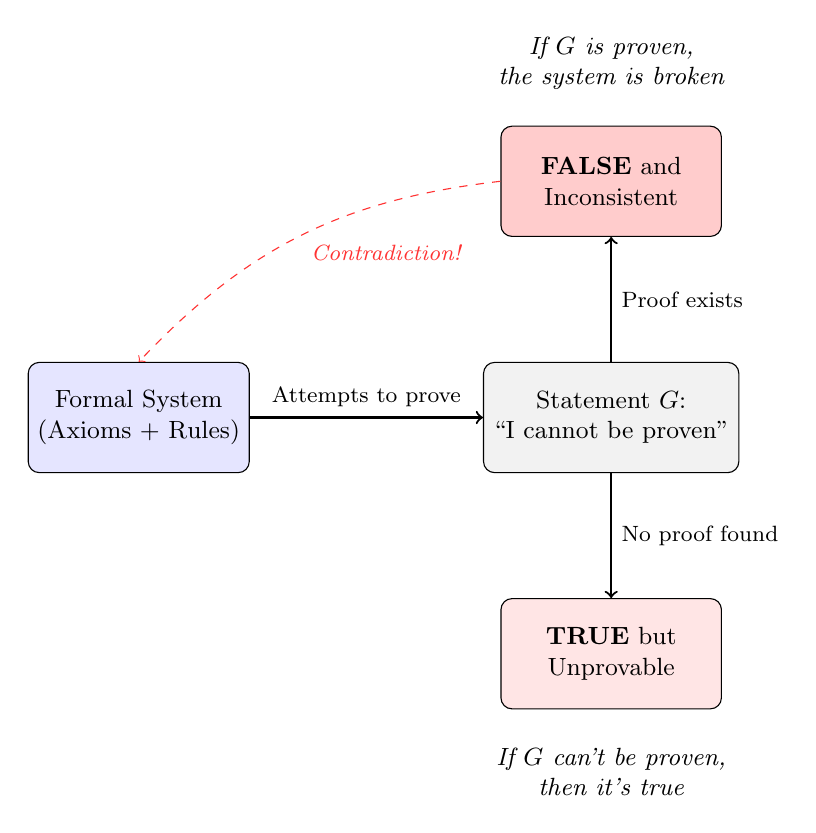
\begin{tikzpicture}[
  every node/.style={font=\small},
  box/.style={draw, rounded corners, minimum width=2.8cm, minimum height=1.4cm, align=center},
  arrow/.style={->, thick}
]

% Nodes
\node[box, fill=blue!10] (system) at (0, 0) {Formal System\\(Axioms + Rules)};
\node[box, fill=gray!10] (G) at (6, 0) {Statement $G$:\\``I cannot be proven''};
\node[box, fill=red!10] (true) at (6, -3) {\textbf{TRUE} but \\ Unprovable};
\node[box, fill=red!20] (false) at (6, 3) {\textbf{FALSE} and\\ Inconsistent};

% Arrows
\draw[->, thick] (system.east) -- node[above] {\footnotesize Attempts to prove} (G.west);
\draw[->, thick] (G.south) -- node[right] {\footnotesize No proof found} (true.north);
\draw[->, thick] (G.north) -- node[right] {\footnotesize Proof exists} (false.south);

% Annotations
\node[align=center, font=\small\itshape] at (6, -4.5) {If $G$ can't be proven, \\ then it's true};
\node[align=center, font=\small\itshape] at (6, 4.5) {If $G$ is proven, \\ the system is broken};

% Optional arrows showing paradox
\draw[->, dashed, red!80] (false.west) to[bend left=-20] node[below right, font=\footnotesize\itshape] {Contradiction!} (system.north);

\end{tikzpicture}
\caption{Gödel’s paradox: $G$ creates a loop where proving it breaks the system, and failing to prove it makes it true.}
\end{figure}

\vspace{1em}









\medskip

\subsubsection{The Deeper Implication: Truth and Proof Are Not the Same}

Before Gödel, many believed that truth and provability were the same thing. If a statement was true, then surely a clever enough person (or machine) could prove it, given enough time.

Gödel shattered that illusion.

There are true mathematical statements that we will never prove — not because we’re not clever enough, but because the system itself simply can’t reach them.

\medskip

\noindent\textbf{So what died with Gödel’s theorem?} Not mathematics. But certainty. The hope for a perfect, airtight foundation collapsed.

\begin{quote}
The monster wasn’t in the axioms. It was in the mirror.
\end{quote}


\begin{tcolorbox}[colback=blue!5!white, colframe=blue!50!black, 
  title={Historical Sidebar: Gödel and Hilbert—The Dream and the Detonation}]
  
  \textbf{David Hilbert} was the optimist of logic. At the dawn of the 20th century, he dreamed of a grand unification: a complete, consistent, and computable foundation for all of mathematics. He called it the \textbf{“formalist program”}—and he meant to prove, once and for all, that math was bulletproof.
  
  \medskip
  
  \textbf{Kurt Gödel} didn’t mean to kill the dream. But in 1931, that’s exactly what he did.
  
  Using a brilliant self-referential trick—essentially building a statement that says “this statement is unprovable”—Gödel proved that any sufficiently powerful formal system (like arithmetic) is either \textbf{incomplete} or \textbf{inconsistent}. You can’t have both completeness and soundness. Some truths, it turns out, will always live outside the system.
  
  \medskip
  
  Hilbert’s rallying cry was “\textit{Wir müssen wissen — wir werden wissen!}”  
  \emph{“We must know—and we will know!”}  
  Gödel’s theorems added a haunting footnote:  
  \emph{We must know... but some things we never can.}
  
  \medskip
  
  To be clear: Gödel didn’t think mathematics was broken—he believed in a higher, Platonic truth. But his work revealed that no formal system could ever fully contain it. The dream of mathematics as a perfect machine was over.
  
  \medskip
  
  \textbf{Hilbert gave us the blueprint. Gödel lit the fuse.}
  
\end{tcolorbox}


\subsection{Infinity Strikes Back}

Gödel’s theorem didn’t just upend logic; it threw a Molotov cocktail into the already-smoldering debate about infinity. At the heart of the firestorm was the \textbf{Continuum Hypothesis (CH)}:

\begin{quote}
Is there an infinity between the size of the natural numbers () and the real numbers ()?
\end{quote}

Cantor had suspected the answer was no. Hilbert made proving or disproving CH the first challenge of the 20th century. But then Gödel and Cohen came along and pulled the rug out:

\begin{itemize}
\item Gödel showed that CH \textbf{cannot be disproven} using standard set theory (ZFC).
\item Cohen then showed that CH \textbf{cannot be proven} either.
\end{itemize}

Which meant that the truth of CH wasn’t just unknown—it was \textit{unknowable}. You could assume CH was true. You could assume it was false. \textbf{Both were equally valid.} Welcome to the multiverse of mathematical reality.

\subsection{When Incompleteness Meets Information: Vitali Sets, Signals, and the Limits of Sampling}

\subsubsection{How This Changed Integration Forever}

This wasn’t just a problem for set theorists arguing in dimly lit offices. It had real consequences for how we define \textbf{measure and integration}. Thanks to Gödel, we now know that the sets we assign measure to—the ones we integrate over—are not uniquely determined by logic.

Instead, we have \textbf{choices}. Different models of mathematics allow for different sets to be measurable, and all of them are “correct” within their chosen framework. The question of \textbf{which infinities we allow to have size} is no longer a matter of proof—it’s a matter of preference.

Cantor may have broken mathematics, but Gödel made sure the pieces would never fit back together. 

\subsubsection{When Incompleteness Meets Information: Vitali Sets}

To understand how Gödel’s incompleteness theorem and the Continuum Hypothesis affect modern information theory, we need to revisit one of the strangest objects in mathematics: the \textbf{Vitali set}.

In 1905, the Italian mathematician \textbf{Giuseppe Vitali} used the Axiom of Choice to prove that there exists a subset of the real numbers that is \emph{not} Lebesgue measurable. His construction went like this:

\begin{itemize}
  \item Consider the interval \([0,1]\), and define an equivalence relation where two numbers \( x \sim y \) if \( x - y \) is rational.
  \item This partitions \([0,1]\) into uncountably many disjoint equivalence classes.
  \item Using the Axiom of Choice, select exactly one representative from each class. The resulting set is called a \textbf{Vitali set}.
\end{itemize}

\begin{figure}[H]
\centering
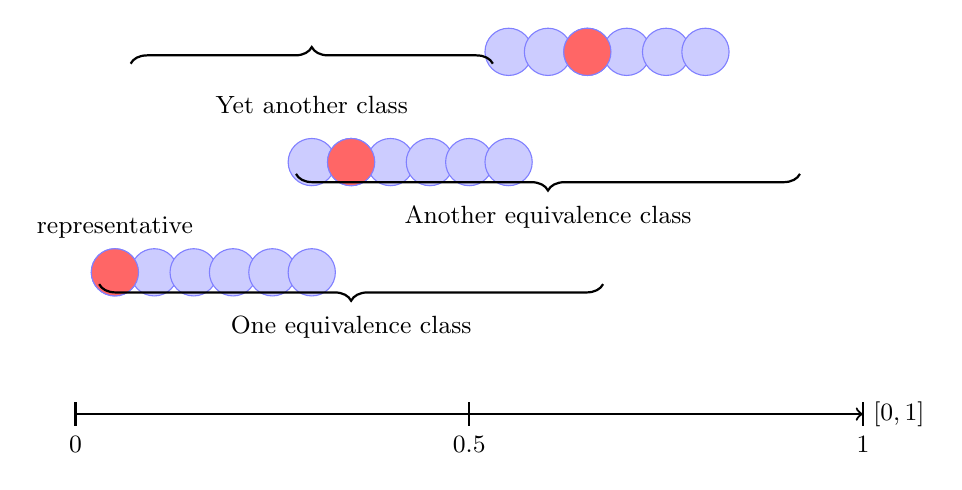
\begin{tikzpicture}[
  every node/.style={font=\small},
  class/.style={circle, fill=blue!20, draw=blue!50, minimum size=0.6cm, inner sep=0pt},
  rep/.style={class, fill=red!60},
  axis/.style={thick, ->},
  tick/.style={thick}
]

% Draw the interval [0,1]
\draw[axis] (0,0) -- (10,0) node[right] {\( [0,1] \)};
\foreach \x/\label in {0/0, 5/0.5, 10/1}
  \draw[tick] (\x,0.15) -- (\x,-0.15) node[below] {\(\label\)};

% Partition dots (rational offsets) — added vertical spacing
\foreach \i/\x in {1/0.5, 2/1.0, 3/1.5, 4/2.0, 5/2.5, 6/3.0}
{
  \node[class] (c\i1) at (\x, 1.8) {};
  \node[class] (c\i2) at ({mod(\x+2.5,10)}, 3.2) {};
  \node[class] (c\i3) at ({mod(\x+5.0,10)}, 4.6) {};
}

% Representatives
\node[rep, label=above:{representative}] at (0.5,1.8) {};
\node[rep] at (3.5,3.2) {};
\node[rep] at (6.5,4.6) {};

% Braces and labels for classes — spaced vertically
\draw[decorate,decoration={brace,mirror,amplitude=6pt}, thick] (0.3,1.65) -- (6.7,1.65) node[midway, below=8pt] {One equivalence class};
\draw[decorate,decoration={brace,mirror,amplitude=6pt}, thick] (2.8,3.05) -- (9.2,3.05) node[midway, below=8pt] {Another equivalence class};
\draw[decorate,decoration={brace,mirror,amplitude=6pt}, thick] (5.3,4.45) -- (0.7,4.45) node[midway, below=8pt] {Yet another class};

\end{tikzpicture}
\caption{Constructing the Vitali set: choose one point from each rational-shifted equivalence class within \([0,1]\). This set defies Lebesgue measure.}
\end{figure}

\medskip

To understand how strange this is, think about how we normally measure subsets of the real line. If you shift a set to the left or right, its length stays the same—this is called translation invariance. If you break a set into countably many disjoint parts and measure each one, their lengths should add up: this is countable additivity. 

\begin{quote}
If a set is well-behaved in a certain technical sense (i.e., Borel or Lebesgue measurable), then we say it’s complete with respect to the measure. And, the Vitali set breaks all of these intuitions.
\end{quote}

It’s not that we don’t know how to measure it. It’s that we provably can’t—not without violating at least one of the axioms that make Lebesgue measure work. If you try to assign it a length, you’ll quickly run into contradictions: either you lose translation invariance, or you give up countable additivity, or your measure becomes incomplete.

\begin{figure}[H]
\centering
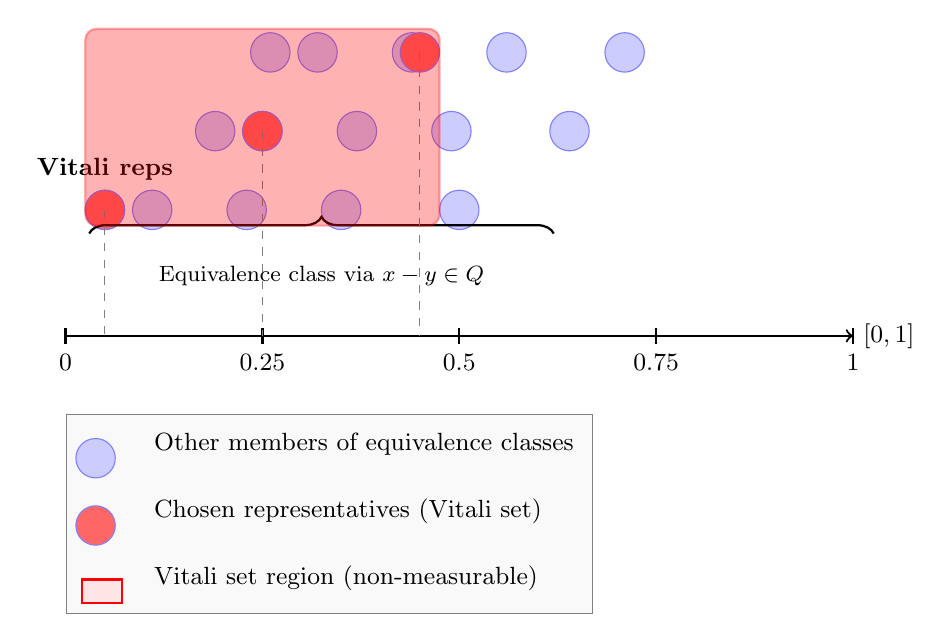
\begin{tikzpicture}[
  every node/.style={font=\small},
  class/.style={circle, fill=blue!20, draw=blue!50, minimum size=0.5cm, inner sep=0pt},
  rep/.style={class, fill=red!60},
  axis/.style={thick, ->},
  tick/.style={thick}
]

% Draw the interval [0,1]
\draw[axis] (0,0) -- (10,0) node[right] {\( [0,1] \)};
\foreach \x/\label in {0/0, 2.5/0.25, 5/0.5, 7.5/0.75, 10/1}
  \draw[tick] (\x,0.1) -- (\x,-0.1) node[below] {\(\label\)};

% Rational translations (classes)
\foreach \i/\x in {1/0.5, 2/1.1, 3/2.3, 4/3.5, 5/5.0}
{
  \node[class] (c\i1) at ({mod(\x,10)}, 1.6) {};
  \node[class] (c\i2) at ({mod(\x+1.4,10)}, 2.6) {};
  \node[class] (c\i3) at ({mod(\x+2.1,10)}, 3.6) {};
}

% Representatives
\node[rep, label=above:{\textbf{Vitali reps}}] at (0.5,1.6) {};
\node[rep] at (2.5,2.6) {};
\node[rep] at (4.5,3.6) {};

% Braces and annotations
\draw[decorate,decoration={brace,amplitude=6pt}, thick] (0.3,1.3) -- (6.2,1.3) node[midway, below=8pt] {\footnotesize Equivalence class via \(x - y \in \mathbb{Q}\)};
\draw[dashed, gray] (0.5,1.6) -- (0.5,0);
\draw[dashed, gray] (2.5,2.6) -- (2.5,0);
\draw[dashed, gray] (4.5,3.6) -- (4.5,0);

% Vitali set region (implicit)
\draw[fill=red!10, rounded corners, thick, red, opacity=0.3] (0.25,1.4) rectangle (4.75,3.9);

% LEGEND (scaled down)
\begin{scope}[scale=0.66, shift={(0,-1.5)}]
\matrix[draw=black!50, fill=gray!5, column sep=8pt, row sep=4pt, anchor=north west] {
  \node[class] {}; & \node[anchor=west]{Other members of equivalence classes}; \\
  \node[rep] {};   & \node[anchor=west]{Chosen representatives (Vitali set)}; \\
  \node[fill=red!10, minimum width=0.5cm, minimum height=0.3cm, draw=red, thick] {}; & \node[anchor=west]{Vitali set region (non-measurable)}; \\
};
\end{scope}

\end{tikzpicture}
\caption{The Vitali set: by selecting one representative from each rational-translation equivalence class in \([0,1]\), we construct a set that is fundamentally non-measurable. The legend shows how the construction is visualized.}
\end{figure}

In other words: the Vitali set is a kind of mathematical ghost. It “exists” (if you accept the Axiom of Choice), but it refuses to behave. It lurks outside the bounds of what our mathematical tools can grasp cleanly—just like Gödel’s incompleteness theorem shows that some truths exist outside the bounds of what formal systems can prove.

\subsubsection{Why the Vitali Set Is Like an Impossible Signal Sample}

To appreciate the implications of the Vitali set in the world of signal processing, imagine you're working with a digital audio signal. In practice, we sample a continuous waveform at regular intervals—say, 44,100 times per second for CD-quality audio. Each of these samples is a number we can store, process, and analyze.

Now suppose you had a “signal” defined by a Vitali set—where the values exist, but are chosen using the Axiom of Choice in a way that defies any measurable structure. What would that mean?

\begin{itemize}
  \item You couldn’t average its values over any interval—because there's no well-defined way to integrate or sum them.
  \item You couldn’t apply a Fourier transform—because there’s no consistent way to define energy or frequency content.
  \item You couldn’t even plot it meaningfully—because it resists being described in terms of measurable functions.
\end{itemize}

\textbf{Bottom line:} If Lebesgue measure is your ruler, then the Vitali set is a shape that shatters it. And in domains like signal processing, where measurement and structure are everything, that’s a serious philosophical curveball.


\begin{quote}
In signal processing terms, the Vitali set is like a waveform that has no frequency, no amplitude, no duration, and no structure—yet still “exists” on paper. It’s a theoretical object that breaks every tool you’d normally use to understand or manipulate signals.
\end{quote}


\textbf{In other words:} the success of Shannon's sampling theorem depends entirely on the assumption that the signal lives in a well-behaved mathematical universe—one where 

\begin{enumerate}
	\item integration makes sense, 
	\item Fourier transforms converge, and 
	\item the measure of a set is a meaningful quantity. 
\end{enumerate}

The moment you step outside that universe, things fall apart.





\begin{figure}[H]
\centering
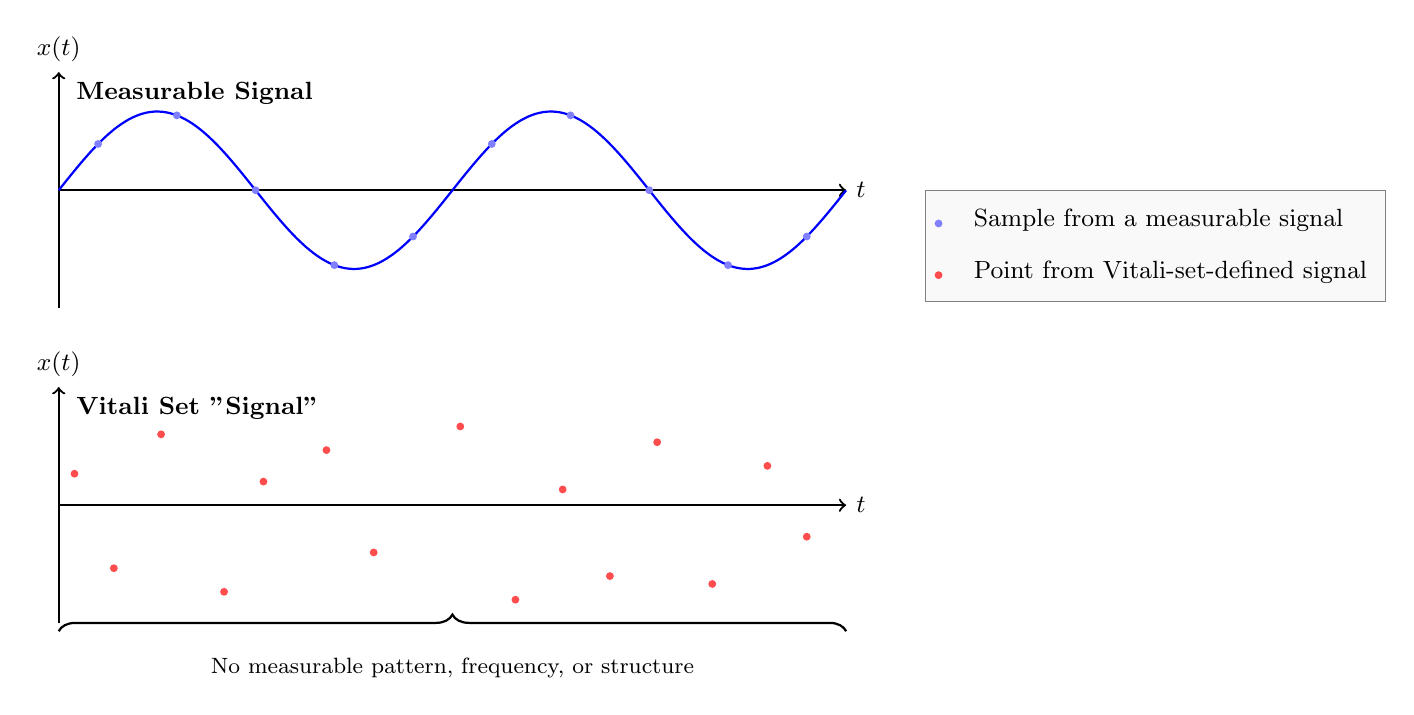
\begin{tikzpicture}[
    every node/.style={font=\small},
    axis/.style={->, thick},
    sample/.style={circle, fill=blue!50, inner sep=1pt},
    vitali/.style={circle, fill=red!70, inner sep=1pt},
    chaos/.style={draw=none, fill=red!20, minimum width=0.15cm, minimum height=0.6cm}
]

% Axis for measurable signal
\draw[axis] (0,0) -- (10,0) node[right] {\( t \)};
\draw[axis] (0,-1.5) -- (0,1.5) node[above] {\( x(t) \)};
\node[anchor=north west] at (0.1,1.5) {\textbf{Measurable Signal}};

% Draw sinusoid
\draw[thick, blue, domain=0:10, samples=100, smooth] plot(\x,{sin(2*pi*\x/5 r)});

% Sample points
\foreach \x in {0.5,1.5,...,9.5}
    \node[sample] at (\x,{sin(2*pi*\x/5 r)}) {};

% Axis for Vitali signal
\begin{scope}[yshift=-4cm]
\draw[axis] (0,0) -- (10,0) node[right] {\( t \)};
\draw[axis] (0,-1.5) -- (0,1.5) node[above] {\( x(t) \)};
\node[anchor=north west] at (0.1,1.5) {\textbf{Vitali Set "Signal"}};

% Chaos dots - unpredictable pattern
\foreach \x/\y in {
    0.2/0.4, 0.7/-0.8, 1.3/0.9, 2.1/-1.1, 2.6/0.3,
    3.4/0.7, 4.0/-0.6, 5.1/1.0, 5.8/-1.2, 6.4/0.2,
    7.0/-0.9, 7.6/0.8, 8.3/-1.0, 9.0/0.5, 9.5/-0.4
}
    \node[vitali] at (\x,\y) {};

% Annotate chaos zone
\draw[decorate,decoration={brace,amplitude=6pt}, thick] (0,-1.6) -- (10,-1.6) node[midway, below=6pt] {\footnotesize No measurable pattern, frequency, or structure};

\end{scope}

% Legend
\begin{scope}[shift={(11,0)}]
\matrix[draw=black!50, fill=gray!5, column sep=8pt, row sep=4pt, anchor=north west] {
  \node[sample] {}; & \node[anchor=west]{Sample from a measurable signal}; \\
  \node[vitali] {}; & \node[anchor=west]{Point from Vitali-set-defined signal}; \\
};
\end{scope}

\end{tikzpicture}
\caption{Top: a standard sinusoidal signal with well-defined samples. Bottom: a hypothetical signal defined by a Vitali set — unstructured, non-integrable, and incompatible with standard signal processing tools.}
\end{figure}


\vspace{1em}

\subsubsection{Why the Vitali Set Breaks Signal Processing}

A function defined over a Vitali set may technically exist, but it's not something we can sample, analyze, or reconstruct. There is no meaningful way to define its average value over any interval, because those intervals contain unmeasurable subsets. There is no total energy, because the integral that would define it can't be evaluated. Even the idea of plotting it—visualizing it on a screen—becomes meaningless, because the signal doesn't exist over a structure that supports length, area, or continuity.

This is where Gödel and Vitali collide with information theory. \textbf{Not all functions are reconstructible. Not because we lack bandwidth or resolution—but because, in a deep mathematical sense, some signals simply defy structure.} They live in logical shadows: formally present, but physically inaccessible.

So while Shannon showed us how to digitize the infinite, Vitali reminds us that some parts of the infinite are beyond digitization altogether.

\begin{quote}
Sampling assumes measurability. Vitali sets exist to show what happens when you take that away.
\end{quote}

Now here’s where things get weird: whether or not Vitali sets (and other non-measurable monsters) exist depends on your set-theoretic universe. If you assume the Continuum Hypothesis and the Axiom of Choice, these sets exist. But if you reject CH and adopt determinacy axioms instead, \emph{every subset of \(\mathbb{R}\) becomes measurable}.

This might sound like a philosophical nuisance—until you realize that it has real implications for how we define and manipulate functions in information theory.

But the notion of “integrable” here depends on Lebesgue measure, which in turn assumes we’re only dealing with \emph{measurable} functions.

But what if the “signal” we’re trying to reconstruct includes a Vitali set in its support? Or worse, what if the underlying probability distribution (over which we compute entropy) is defined on a non-measurable subset of the reals?

\begin{itemize}
  \item Under some models (CH + Axiom of Choice), such sets exist and break our assumptions about integration.
  \item Under other models (¬CH + Determinacy), these pathologies vanish: all sets are measurable, and entropy is always well-defined.
\end{itemize}

This means that your ability to \textbf{measure uncertainty, define entropy, or reconstruct a signal} can depend on which version of set theory you believe in.

\vspace{1em}
\textbf{Gödel’s Theorem and the Unknowability of Measurement}

Gödel’s incompleteness theorem ensures that questions like the Continuum Hypothesis cannot be settled from within standard mathematics (ZFC). That means whether Vitali-like sets exist is not just unknown—it’s \emph{unknowable}.

And so, ironically, even though information theory was born to measure uncertainty, we now know that there are forms of uncertainty it \emph{cannot measure}—not due to noise or lack of data, but due to the foundational limits of mathematics itself.

\begin{quote}
\textbf{The lesson:} Information theory may tell us how to transmit, compress, and recover data—but Gödel and Cantor remind us there are questions even perfect data can’t answer.
\end{quote}


\begin{example}[title={When Entropy Breaks: A Distribution on a Vitali Set}]
Let’s say you want to define a random variable \( X \) that takes values in the interval \([0,1]\), and you want to compute its entropy:
\[
H(X) = -\int_{[0,1]} p(x) \log_2 p(x)\, dx
\]
\\
This works perfectly—\emph{if} \( p(x) \) is defined over a measurable subset of \([0,1]\). But now suppose we define \( X \) to be “uniform” over a \textbf{Vitali set} \( V \subset [0,1] \):
\begin{itemize}
  \item Let \( p(x) = c \) for \( x \in V \), and 0 otherwise.
  \item Choose \( c \) so that \( \int_V p(x)\, dx = 1 \).
\end{itemize}
\ \\
Here’s the problem:
\begin{itemize}
  \item The set \( V \) is \emph{not} Lebesgue measurable.
  \item The integral \( \int_V p(x)\, dx \) is undefined.
  \item Therefore, \( H(X) \) cannot be evaluated in any meaningful way.
\end{itemize}
\ \\
\textbf{Conclusion:} If a probability distribution is defined on a non-measurable set, then entropy—along with expectation, variance, and most tools of analysis—completely breaks down. The distribution may “exist,” but it defies integration, structure, and interpretation.
\ \\
\begin{quote}
A probability over a Vitali set isn’t just hard to compute—it’s fundamentally outside the bounds of measurement.
\end{quote}
\end{example}







\subsection{The Continuum Hypothesis: Integration at a Philosophical Crossroads}

If Gödel showed us the boundaries of proof, the Continuum Hypothesis (CH) showed us the boundaries of size—and together, they revealed something far more unsettling.

The CH asks whether there is a set whose cardinality lies strictly between that of the natural numbers (\( \aleph_0 \)) and the real numbers (\( 2^{\aleph_0} \)). In practical terms: is there a “middle-sized” infinity between countable sequences and the continuum of the real line?

But here’s where the math gets metaphysical: your answer to this question can change what it means to \emph{integrate}.

Lebesgue integration—our gold standard for measuring probability, entropy, and signal energy—relies on being able to assign meaningful sizes (measures) to subsets of the real line. And for that, you need to assume something about how many subsets actually exist.

Under CH, there are “just enough” subsets of the reals to allow the construction of non-measurable sets like Vitali sets. These are the mathematical equivalent of black holes—regions where measure breaks down. You can define a function that includes them, but you can’t assign it an integral. It’s like writing down an equation you know you’re not allowed to solve.

But under \( \neg \)CH—especially when paired with determinacy axioms—every set of real numbers becomes measurable. The Vitali set vanishes. The monsters are gone. Integration is safe again.

In this light, the Continuum Hypothesis becomes more than an abstract question about infinities—it becomes a referendum on the very foundations of integration. Do we live in a universe where some functions can’t be integrated, not because they’re wild or infinite, but because the underlying set theory refuses to allow their area to exist?

This is why Gödel and Cohen’s results shook analysis to its core. They didn’t just tell us the Continuum Hypothesis was undecidable—they told us integration itself depends on how you answer it.

\vspace{1em}
\textbf{So what does this mean for analysts, physicists, and engineers?}

In practice, nothing breaks. We live in a world where the sets we sample, measure, and compute are tame. The signals we analyze don’t contain Vitali sets. The probability distributions we estimate don’t depend on the Axiom of Choice.

But in principle, everything is up for grabs.

When we write an integral, we’re not just summing values—we’re making a commitment. A commitment to a set-theoretic universe where that sum makes sense. And thanks to the Continuum Hypothesis, we now know there’s more than one such universe.

\begin{quote}
\textbf{So when we integrate, we do so with fingers crossed—hoping we’re in the right reality.}
\end{quote}

And that’s not just a footnote to mathematics. That’s the foundation beneath our definitions of energy, entropy, probability, and information. Gödel told us some truths can’t be proven. The Continuum Hypothesis tells us some areas can’t be measured—unless we choose the right version of the infinite.








\begin{figure}[H]
\centering
\begin{tikzpicture}[every node/.style={font=\footnotesize}]

% Panel 1 — Lebesgue starts strong
\comicpanel{0}{4}
  {Lebesgue}
  {Gödel}
  {\textbf{Lebesgue:} You can't integrate over the Vitali set. It’s not measurable. That’s the whole point.}
  {(0,-0.5)}

% Panel 2 — Gödel being mysterious
\comicpanel{7}{4}
  {Gödel}
  {Lebesgue}
  {\textbf{Gödel:} In some models, it exists. In others, it doesn’t. Truth is model-dependent now.}
  {(0,-0.5)}

% Panel 3 — Cohen enters the chat
\comicpanel{0}{0}
  {Cohen}
  {Gödel and Lebesgue}
  {\textbf{Cohen:} Look, I added new sets and CH broke. No more fixed reality. Welcome to the multiverse.}
  {(0,0.8)}

% Panel 4 — Lebesgue loses it
\comicpanel{7}{0}
  {Lebesgue}
  {Cohen and Gödel}
  {\textbf{Lebesgue:} \textit{I just wanted to measure area. Now you're telling me reality is optional?}}
  {(0,0.6)}

\end{tikzpicture}
\caption{
A historical aside: when Gödel and Cohen broke certainty, even Lebesgue had to admit that some integrals are hostage to set theory.
}
\end{figure}













\subsection{Gödel, Wittgenstein, and the Existential Comedy of Math}

By now, you might be wondering: how did Gödel feel about all this? Did he sit back and chuckle while mathematicians ran headfirst into walls he built with pure logic?

Not exactly. Gödel was deeply serious, even spiritual, about mathematics. He believed mathematical truths were as real as stars or atoms—just harder to find. To him, incompleteness wasn’t a flaw in math; it was a revelation. A warning label stamped on the foundations of thought: “There are truths you will never reach, no matter how clever you are.”

\noindent Wittgenstein, on the other hand, read Gödel’s paper and famously declared it nonsense. He thought it was all a linguistic trick—that Gödel hadn’t discovered anything deep about mathematics, just about the weird ways we talk about it.

\medskip

\noindent This clash wasn’t just academic; it was personal and philosophical. Wittgenstein had once been seen as a kind of prophet by the logical positivists. His early work, the \emph{Tractatus Logico-Philosophicus}, outlined a vision of the world built from logical ``atoms'': a theory known as \textbf{logical atomism}. The Vienna Circle revered him. They saw in his work the blueprint for a purified language of science and mathematics, stripped of ambiguity.

But Wittgenstein changed his mind. In his later years, he rejected the idea of rigid logical structures as the foundation of meaning. Instead, he proposed that meaning comes from \textbf{language games}: the social, contextual use of language in specific settings. In this view, mathematics wasn’t a realm of Platonic truth, but just one more game we play with symbols and rules.

Gödel, meanwhile, had been loosely connected to the Vienna Circle but stood apart in temperament and conviction. While the Circle emphasized empiricism and verification, Gödel believed in a deep, Platonic reality behind mathematics --- truths that existed independently of our proofs or perceptions.

Gödel didn’t just publish a theorem—he detonated a philosophical bomb under the foundations of logic itself. His incompleteness results so thoroughly shattered the dreams of the logical positivists that the entire landscape of 20th-century thought shifted in response. The Vienna Circle had hoped for a crystalline, complete language of science grounded in logic, but Gödel showed that even arithmetic—logic’s supposed bedrock—contained truths that logic alone could never reach. The fallout was existential. Wittgenstein, once their intellectual lodestar, pivoted from logical atomism to language games, drifting toward a postmodernist view where meaning was social, not structural. Popper, seeking stability, offered falsification in place of verification. Others, like Quine and later pragmatists, abandoned the idea of foundational knowledge altogether, embracing the contingency of belief systems and the shifting utility of models. 

\begin{quote}
And so we’re left, even today, staring at the statue of science and wondering if its gleaming form stands on feet of clay.
\end{quote}


This sparked one of the most quietly savage standoffs in intellectual history. Gödel, the shy logician who could barely give a lecture without collapsing from stress. Wittgenstein, the brooding philosopher who once waved a fireplace poker at Karl Popper while debating the merits of falsification. Each thought the other was missing the point. 

And the rest of the math world? It fractured into four tribes:

\begin{itemize}
    \item The \textbf{Formalists} shrugged and said, “Let’s just keep proving stuff and hope the roof doesn’t collapse.”
    \item The \textbf{Intuitionists} muttered, “Told you so,” and went off to live in a hut where infinity doesn’t exist.
    \item The \textbf{Platonists} raised a glass to Gödel, muttering, “The Truth is out there,” like mathematical Mulder cultists.
    \item The \textbf{Pragmatists} said, “Does it run on silicon? Good enough for us.”
\end{itemize}


\vspace{1em}

\begin{tcolorbox}[colback=blue!5!white, colframe=blue!50!black, title=Historical Sidebar: Truth vs Games]

  \textbf{Kurt Gödel} believed that mathematical truths were \emph{real}. Not “useful” or “agreed upon” or “symbolically convenient”—real, as in floating somewhere in a timeless Platonic realm. His incompleteness theorems weren’t just technical results; they were existential declarations: \emph{Some truths are forever beyond formal proof.}
  
  \medskip
  
  \textbf{Ludwig Wittgenstein} wasn’t impressed.  He read Gödel’s theorem and decided it wasn’t metaphysical insight—it was a linguistic misunderstanding. To him, mathematics was a \textbf{language game}: a structured way we talk and reason, shaped by context and use. If your system can’t prove something, maybe you’re just playing the wrong game.
  
  \medskip
  
  Where Gödel saw revelation, Wittgenstein saw confusion. Gödel said, “There are truths you’ll never prove.” Wittgenstein replied, “Define ‘truth.’”
  
  \medskip
  
  Their philosophical tension came to a head during a now-legendary seminar in Cambridge, where Wittgenstein dismissed Gödel’s theorem \emph{without reading it fully}, claiming it was a trick of syntax masquerading as depth. Gödel, shy and soft-spoken, never responded publicly. But privately? He was horrified. He thought Wittgenstein had missed the point entirely.
  
  \medskip
  
  \textbf{The result?} A stalemate worthy of the ages.  Gödel thought mathematics was a window into the eternal.  Wittgenstein thought it was a mirror reflecting our rules.  And neither could convince the other that they were even playing the same game.
  
  \medskip
  
  \textbf{Legacy:}  
  If you're a Platonist, Gödel is your tragic prophet.  If you're a Post-Modernist, Wittgenstein is your knight in shinning armor. If you're a working mathematician, you probably just want your grant proposals approved and your journal articles accepted.
  
\end{tcolorbox}

\vspace{1em}


As for me?

There’s something poetic about it. We built an entire science to measure uncertainty, only to discover that some uncertainties measure us back. We wanted to calculate everything, and found a ceiling made of questions. And somewhere in the basement of the universe, a Vitali set is laughing quietly, unmeasurable and smug.

Math didn’t fail. It just blinked. And Gödel, pale and precise, is still standing in the doorway, whispering:

\begin{quote}
“There’s more than you can ever prove—and less than you’ll ever know.”
\end{quote}



\begin{figure}[H]
\centering

% === First row ===
\begin{subfigure}[t]{0.45\textwidth}
\centering
\begin{tikzpicture}
  \comicpanel{0}{0}
    {Gödel}
    {}
    {\footnotesize There are truths no system can prove. We can’t cage the truth.}
    {(0,-0.6)}
\end{tikzpicture}
\caption*{The incompleteness bomb drops.}
\end{subfigure}
\hfill
\begin{subfigure}[t]{0.45\textwidth}
\centering
\begin{tikzpicture}
  \comicpanel{0}{0}
    {Popper}
    {}
    {\footnotesize Then let’s stop proving and start falsifying. We learn by failure.}
    {(0,-0.6)}
\end{tikzpicture}
\caption*{Science pivots to survival.}
\end{subfigure}

\vspace{1em}

% === Second row ===
\begin{subfigure}[t]{0.45\textwidth}
\centering
\begin{tikzpicture}
  \comicpanel{0}{0}
    {Quine}
    {}
    {\footnotesize Meaning? Truth? Those are just nodes in a semantic web.}
    {(0,-0.6)}
\end{tikzpicture}
\caption*{Goodbye foundations. Hello networks.}
\end{subfigure}
\hfill
\begin{subfigure}[t]{0.45\textwidth}
\centering
\begin{tikzpicture}
  \comicpanel{0}{0}
    {Wittgenstein}
    {}
    {\footnotesize If truth is a game then it’s one I no longer wish to play.}
    {(0,-0.6)}
\end{tikzpicture}
\caption*{Resignation at the edge of reason.}
\end{subfigure}

\caption{The wreckage of certainty: Gödel broke the system, and everyone else rewrote the rules.}
\end{figure}







